\section{Identity and Access Management}

Unter \textbf{Federated Identity Management} gehören Abkommen, Standards und Technologien, um Identitäten und Berechtigungen über autonome Identitätsdomänen zu vereinheitlichen. Die \textit{Föderation} (Zusammenschluss) ermöglicht es, die Identitätsinformationen von verschiedenen Systemen transparent und sicher auszutauschen, um damit auf der Sicherheitsebene zusammenarbeiten zu können.\\

Logindaten und Identitäten sind also nur an einem Ort, dem \textit{Authentity-Provider}, gespeichert und dort findet auch jede Authentifizierung statt. Möchte nun ein fremdes System die Identität prüfen, so wird die Anfrage an den entsprechenden Authentity-Provider weitergeleitet und dessen Antwort abgewartet. Jeder Benutzer kann so einen eigenen Authentity-Provider haben.

\subsection[AAI]{Authentication \& Authorization Infrastructure - AAI}
\textbf{Ohne eine einheitliche AAI} benötigt jede zu schützende Ressource eine separate Benutzer-Administration und -Authentifikation. Probleme / Nachteile ohne AAI:
\begin{easylist}
	& Aufwändige und fehleranfällige Registrierung für jede einzelne Ressource
	& Unzuverlässige und veraltete Daten
	& Verschiedene Login-Prozeduren und Passwörter
	& Gewisse Ressourcen werden gar nicht erst benötigt
	& Ressourcen sind oft nur durch IP-Adressen geschützt
\end{easylist}

\textbf{Mit einer AAI} muss sich der Benutzer nur noch an einer Stelle authentifizieren. Diese kann dann an den verschiedenen Ressourcen für die Autorisierung verwendet werden. Vorteile durch AAI:
\begin{easylist}
	& Keine Registrierung pro Ressource nötig
	& Einheitliche Login-Prozedur
	& Neue Ressourcen können leicht hinzugefügt werden
	& Standortunabhängig
	& Weniger Kennwörter zu merken
\end{easylist}

\begin{figure}[H]
	\centering
	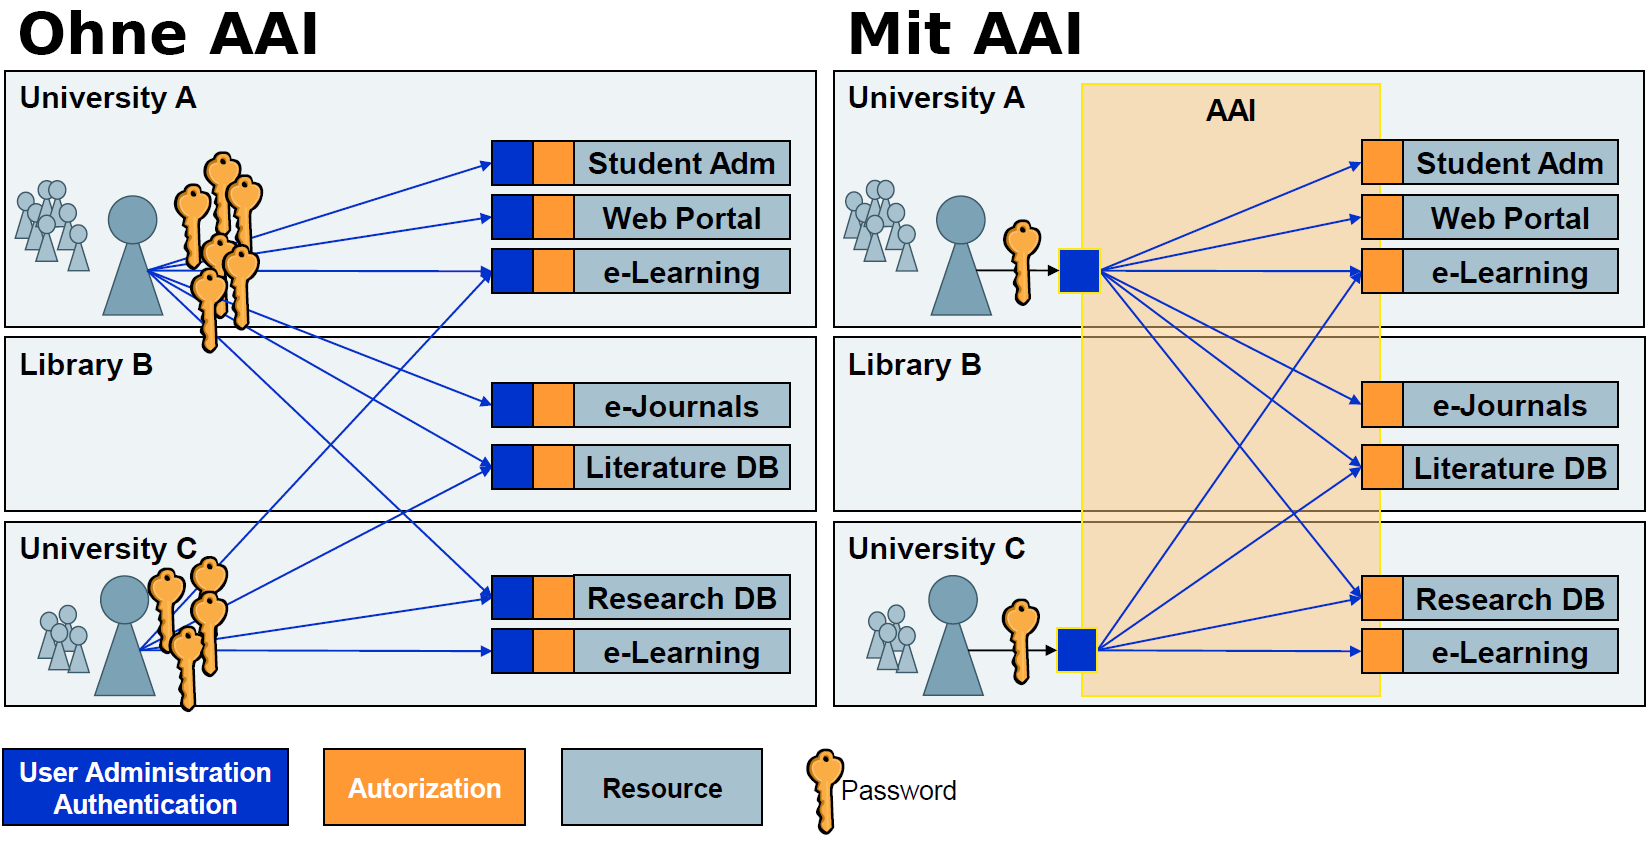
\includegraphics[width=\textwidth]{./img/AAI-example}
	\caption{Exemplarische Übersicht von AAI (Source: switch.ch/aai)}
\end{figure}

\subsubsection{Shibboleth}
Eines der weit verbreitetsten AAI, welches die Authentifizierung von Classic Web-Services über die Protokolle \textbf{SOAP, XML und SAML} übernimmt unter Verwendung von \textbf{http}.\\
Basiert auf \textbf{SAML-Assertions} (\textit{Security Assertion Markup Language}) ausgestellt von vertrauten Home-Organisationen (\textbf{Identity Providers}), welche von Ressourcen (\textbf{Service Providers}) aus dem Verbund akzeptiert werden.

\begin{figure}[H]
	\centering
	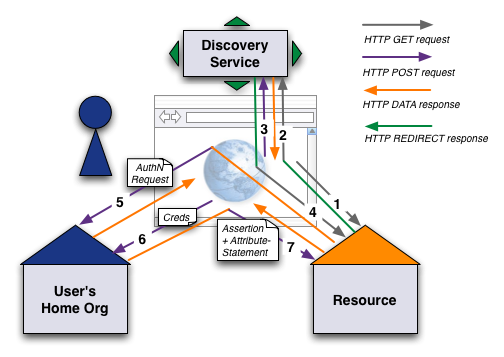
\includegraphics[width=0.7\textwidth]{./img/shibboleth-login}
	\caption{Vollständige Login-Prozedur mit Shibboleth (Source: switch.ch/aai)}
\end{figure}

\textbf{Beispiel}\\
Ein Beispiel für AAI mittels Shibboleth ist das System von SWITCH für Universitäten, mit dem man sich z.B. bei Unterrichtsplattformen oder Online-Shops mit dem Login seiner Uni- / Fachhochschule anmelden kann.\\
Dieses System übermittelt zudem \textbf{zusätzliche Attribute} zum authentifizierten Benutzer, wie etwa seine Mail-Adresse oder SwissEduPersonUniqueID.\\

\textbf{Standards}\\
Der Standard \textbf{XML Signature Syntax and Processing} erlaubt die Signierung, Integritätsprüfung und Nachrichtenauthentifizierung.\\
Der Standard \textbf{XML Encryption Syntax and Processing} erlaubt die Verschlüsselung von Daten innerhalb eines XML-Dokuments.\\
Der Standard \textbf{Secure Assertion Markup Language 2.0} kombiniert \textit{XML Signature Syntax} und \textit{XML Encryption Syntax} in einem Dokument mit Authentifizierung, Attributen und Autorisierung. Das resultierende XML-Dokument ist eine portable Identität für \textbf{Single Sign-On Web Services}.\\
Die Verwendung von SAML bringt als Vorteil mit sich, dass bestehende Enterprise-Anwendungen direkt integriert werden können. Das zugrunde liegende XML bringt aber dennoch etwa \textbf{90\% Overhead} mit sich.\\

Über die Architektur von \textbf{SuisseID} lässt sich so z.B. auch die \textbf{Alters-Verifikation} sicherstellen, da für die Ausstellung eine Identitätsprüfung durchgeführt wird.

\subsubsection{OAuth2}
OAuth2 wurde für neuere Protokolle wie \textbf{REST und JSON} entworfen und kommuniziert über \textbf{https}. Es gibt keine eingebauten Verschlüsselungs-Algorithmen, sondern es wird komplett auf TLS (https) vertraut. Die Funktionsweise ist \textbf{vergleichbar mit Kerberos}.

\begin{description}
	\item[Resource Owner] Benutzer
	\item[Resource Server] Die API
	\item[Authorization Server] Autorisiert den Benutzer (ist oft auf dem selben Server wie \textit{Resource Server})
	\item[Client] Thirt-Party Applikation, welche auf die API zugreifen möchte.
\end{description}

\begin{figure}[H]
	\centering
	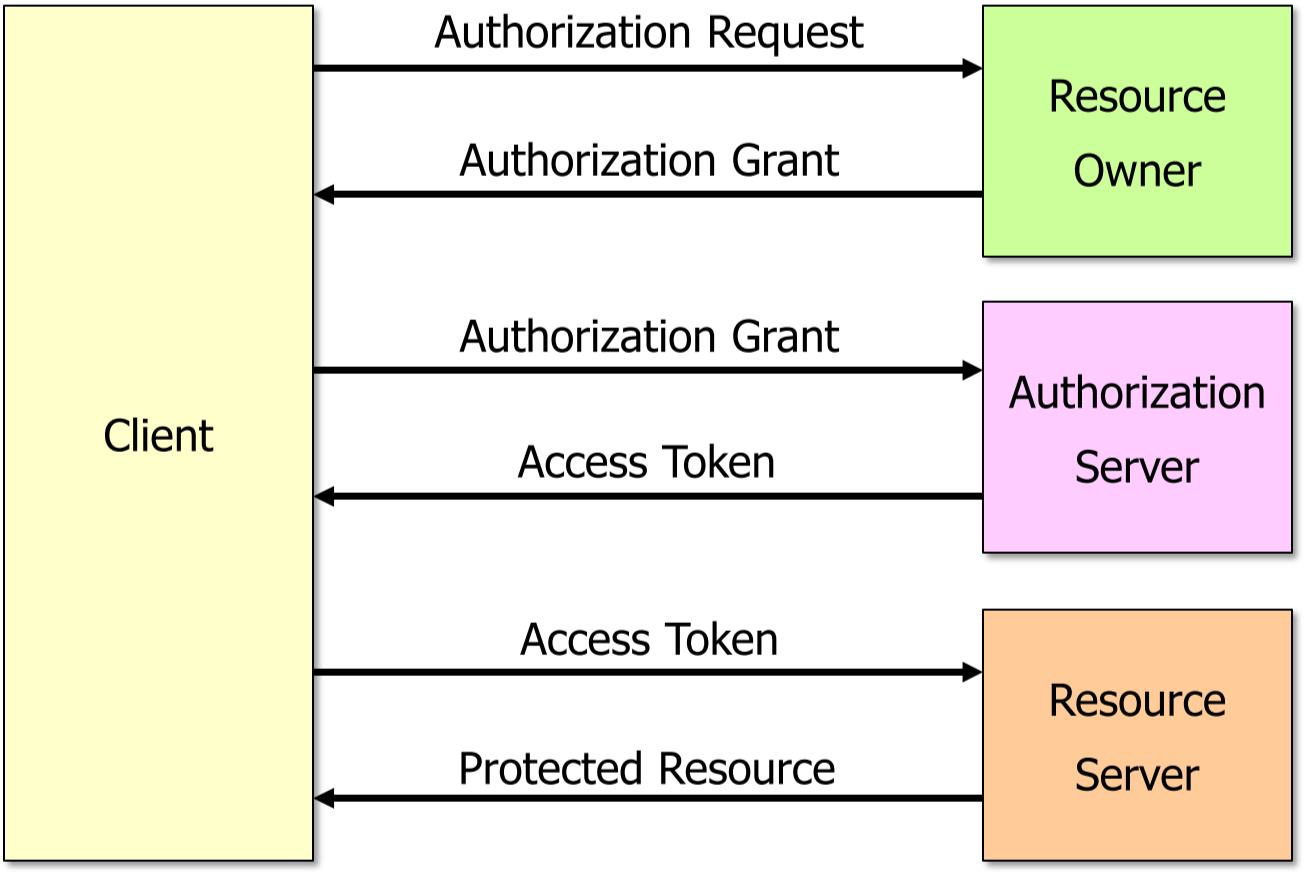
\includegraphics[width=0.5\textwidth]{./img/oauth2-example}
	\caption{Beispiel eines Zugriffs auf geschützte Ressourcen mittels OAuth2}
\end{figure}

Man kann OAuth2 nicht als zuverlässige Benutzerauthentifizierung zählen. \textit{OpenID connect} versucht dieses Problem zu lösen.\\

Jeder Anbieter setzt eine andere Version davon ein oder sogar eine eigene Implementierung.

\subsubsection{OpenID Connect}
\begin{easylist}[itemize]
	& OpenID Connect 1.0 is a simple identity layer on top of OAuth 2.0.
	& OpenID Connect 1.0 specifies a REST-based http API, using JSON as a data format..
	& OpenID Connect 1.0 uses a JSON Web Token (JWT) which can be signed using JSON Web Signature (JWS) and optionally encrypted using JSON Web Encryption (JWE).
	& OpenID Connect 1.0 is used by Google+ Sign-In.
\end{easylist}